\chapter{Introducción. Ondas Gravitacionales}

\section{Motivación y Objetivo}
\section{Representación Ondas Gravitacionales}
\section{Datos utilizados}

Se utilizaron ondas gravitacionales generadas a partir del modelo híbrido \textit{NRHybSur3dq8}\cite{Varma_2019} de relativdad numérica y aproximaciones post Newtonianas para colisiones de agujeros negros binarios.
\\

Cada onda \(h\) generada se representa por una serie temporal compleja de la forma:
\[
h = h_+ + ih_{\times}
\]


Recordando que $h$ está parametrizada por \(\lambda\)

 \[h = h(t; \lambda) = h_{\lambda}(t) = h_{\lambda} \]
 
En este caso \(\lambda\) tendrá 3 dimensiones, $(q, \chi_{1_Z},\chi_{2_Z}) $, y estará acotado de la siguiente manera:

\begin{itemize}
\item Relación entre masas $q$: $1 \le q \le 8$
\item Espín del agujero negro más pesado (liviano) $\chi_{1_Z} (\chi_{1_Z})$: $|\chi_{1_Z}|, |\chi_{2_Z}| < 0.8$
\end{itemize}

\begin{figure}[h]
\centering
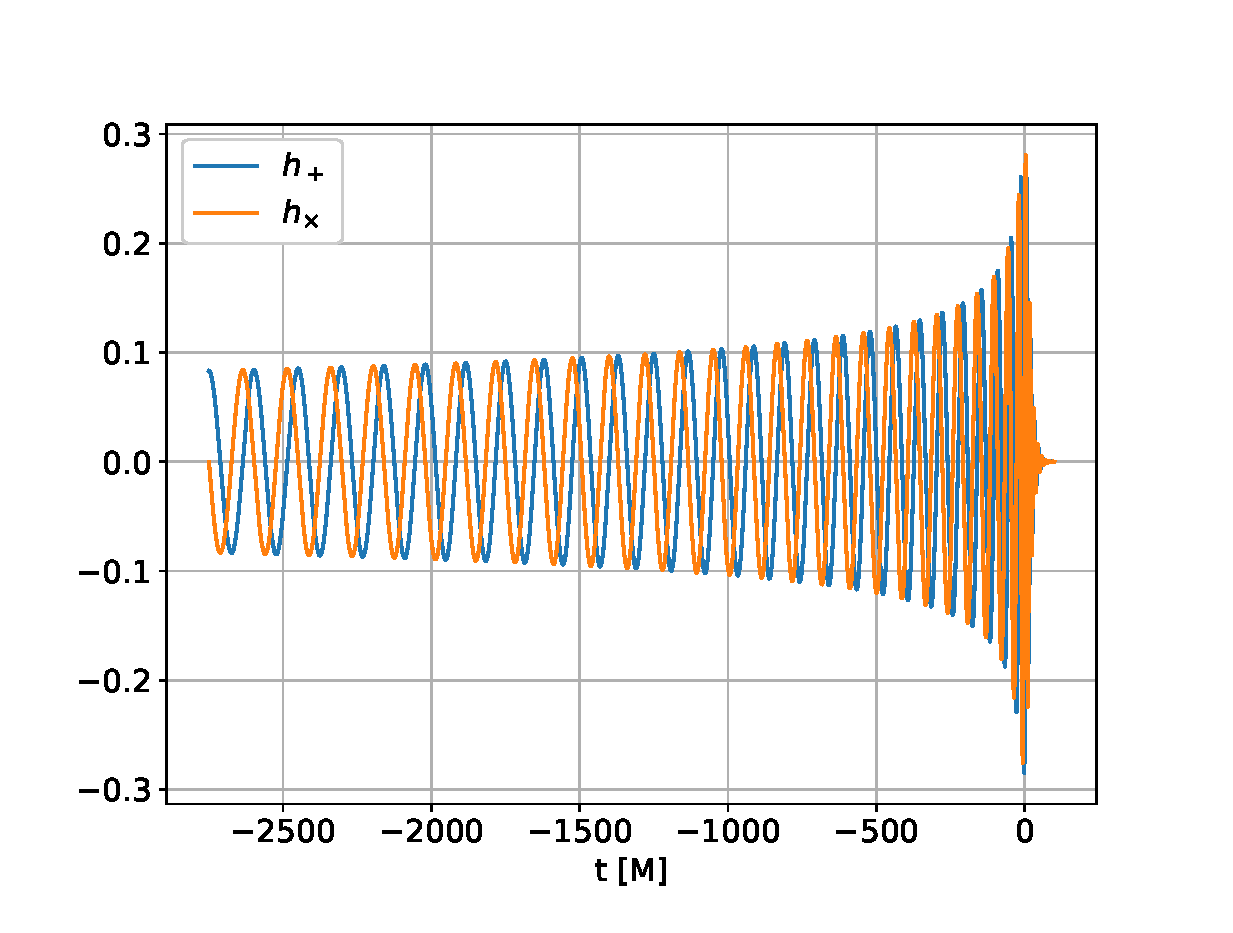
\includegraphics[width=.9\columnwidth]{figs/h_l2m2_q3.eps}
\caption{polarizaciones \(h_+\) y \(h_{\times}\) para $q = 3$, $\chi_{1_Z} = \chi_{2_Z} = 0$, en el modo $l=2$, $m=2$.}
\label{fig:h_q3}
\end{figure}



Se representa un conjunto \( \mathcal{K} \) de N muestras de $\lambda$ de la siguiente forma:

\[ \mathcal{K}  = \{h_{\lambda_i}\}, \hspace{5mm} i = 1, ..., N\]

y debido a que cada $h_{\lambda_i}$ es una serie temporal, se puede representar $\mathcal{K}$ en forma de la matriz $H \in \mathbb{C}^{N\times L}$:

\[
H = 
\begin{bmatrix}
h_{\lambda_1} \\
h_{\lambda_2} \\
 \vdots \\
 h_{\lambda_N} \\
\end{bmatrix}
= 
\begin{bmatrix}
h_{\lambda_1}(t_1) & h_{\lambda_1}(t_2)  & \cdots & h_{\lambda_1}(t_L)\\
 h_{\lambda_2}(t_1) & h_{\lambda_2}(t_2)  & \cdots & h_{\lambda_2}(t_L)\\
 \vdots & \vdots & \ddots &  \vdots \\
h_{\lambda_N}(t_1) & h_{\lambda_N}(t_2)  & \cdots & h_{\lambda_N}(t_L)
\end{bmatrix}
\]

Siendo $L$ la longitud de la serie temporal. De forma que cada fila de $H$ es una onda gravitacional.